\documentclass[a4paper,
fontsize=11pt,
%headings=small,
oneside,
numbers=noperiodatend,
parskip=half-,
bibliography=totoc,
final
]{scrartcl}

\usepackage{synttree}
\usepackage{graphicx}
\setkeys{Gin}{width=.4\textwidth} %default pics size

\graphicspath{{./plots/}}
\usepackage[ngerman]{babel}
\usepackage[T1]{fontenc}
%\usepackage{amsmath}
\usepackage[utf8x]{inputenc}
\usepackage [hyphens]{url}
\usepackage{booktabs} 
\usepackage[left=2.4cm,right=2.4cm,top=2.3cm,bottom=2cm,includeheadfoot]{geometry}
\usepackage{eurosym}
\usepackage{multirow}
\usepackage[ngerman]{varioref}
\setcapindent{1em}
\renewcommand{\labelitemi}{--}
\usepackage{paralist}
\usepackage{pdfpages}
\usepackage{lscape}
\usepackage{float}
\usepackage{acronym}
\usepackage{eurosym}
\usepackage[babel]{csquotes}
\usepackage{longtable,lscape}
\usepackage{mathpazo}
\usepackage[normalem]{ulem} %emphasize weiterhin kursiv
\usepackage[flushmargin,ragged]{footmisc} % left align footnote
\usepackage{ccicons} 
\setcapindent{0pt} % no indentation in captions

%%%% fancy LIBREAS URL color 
\usepackage{xcolor}
\definecolor{libreas}{RGB}{112,0,0}

\usepackage{listings}

\urlstyle{same}  % don't use monospace font for urls

\usepackage[fleqn]{amsmath}

%adjust fontsize for part

\usepackage{sectsty}
\partfont{\large}

%Das BibTeX-Zeichen mit \BibTeX setzen:
\def\symbol#1{\char #1\relax}
\def\bsl{{\tt\symbol{'134}}}
\def\BibTeX{{\rm B\kern-.05em{\sc i\kern-.025em b}\kern-.08em
    T\kern-.1667em\lower.7ex\hbox{E}\kern-.125emX}}

\usepackage{fancyhdr}
\fancyhf{}
\pagestyle{fancyplain}
\fancyhead[R]{\thepage}

% make sure bookmarks are created eventough sections are not numbered!
% uncommend if sections are numbered (bookmarks created by default)
\makeatletter
\renewcommand\@seccntformat[1]{}
\makeatother


\usepackage{hyperxmp}
\usepackage[colorlinks, linkcolor=black,citecolor=black, urlcolor=libreas,
breaklinks= true,bookmarks=true,bookmarksopen=true]{hyperref}
\usepackage{breakurl}

%meta
%meta

\fancyhead[L]{S. Nordhoff\\ %author
LIBREAS. Library Ideas, 35 (2019). % journal, issue, volume.
\href{http://nbn-resolving.de/}
{}} % urn 
% recommended use
%\href{http://nbn-resolving.de/}{\color{black}{urn:nbn:de...}}
\fancyhead[R]{\thepage} %page number
\fancyfoot[L] {\ccLogo \ccAttribution\ \href{https://creativecommons.org/licenses/by/4.0/}{\color{black}Creative Commons BY 4.0}}  %licence
\fancyfoot[R] {ISSN: 1860-7950}

\title{\LARGE{Warum kostet ein wissenschaftliches Buch 28.000\,EUR?}}% title
\author{Sebastian Nordhoff} % author

\setcounter{page}{1}

\hypersetup{%
      pdftitle={Warum kostet ein wissenschaftliches Buch 28.000 EUR?},
      pdfauthor={Sebastian Nordhoff},
      pdfcopyright={CC BY 4.0 International},
      pdfsubject={LIBREAS. Library Ideas, 35 (2019).},
      pdfkeywords={Open Access, Monografien, Language Science Press, Geschäftsmodell, Transparenz, open access books, scholarly communication, business model, transparency},
      pdflicenseurl={https://creativecommons.org/licenses/by/4.0/},
      pdfcontacturl={http://libreas.eu},
      baseurl={http://libreas.eu},
      pdflang={de},
      pdfmetalang={de}
     }



\date{}
\begin{document}

\maketitle
\thispagestyle{fancyplain} 

%abstracts
\begin{abstract}
\noindent \textbf{Abstract}: Dieser Aufsatz bespricht die Kostenstruktur der
Produktion von Open-Access-Büchern und weist auf den derzeitigen Mangel
an belastbaren Zahlen zu den tatsächlichen Kosten der OA-Buchproduktion
hin. Um diesem Mangel abzuhelfen, wird eine gemeinschaftliche
Anstrengung zur offenen Inventarisierung und Bepreisung der
erfordelichen Tätigkeiten gefordert. Eine Referenzimplementierung wird
anhand des Projekts ``Full disclosure: replicable strategies for book
publications supplemented with empirical data'' vorgestellt.
\end{abstract}

%body
Am 13. Juni 2018 veröffentlichte John Sherer von der \emph{Open Access
Monography Initiative} einen Blogpost, der sich der Zukunft der
wissenschaftlichen Monographien und deren Finanzierung in der
Geschichtswissenschaft widmet (Sherer 2018). Unterstützt von der Andrew
W. Mellon Foundation untersucht das Projekt, welche Strategien
Bibliotheken nutzen können, um langfristig die Finanzierung von
Buchpublikationen sicherstellen zu können.

Dabei kommt das Projekt zu folgendem Schluss:

\begin{quote}
\enquote{we've determined that a standard 312-page book that sells 450
copies at a price point of \$40 incurs a loss to the Press of almost
\$14,000.}
\end{quote}

In anderen Worten: Bei Erlösen von 18.000 USD beträgt der Verlust immer
noch 14.000 USD. In der Produktion kostet der Titel also 32.000 USD
(28.000 EUR). Das kann man nun in Arbeitszeit umrechnen. Bei TVÖD E-11
ergeben sich ungefähr sechs Monate Vollbeschäftigung. Diese Zahlen
versetzen Uneingeweihte regelmäßig in Erstaunen. Was könnte man in einem
halben Jahr nicht sonst noch alles anstellen! Das Projekt \enquote{Open
Access History Monograph Initiative} ist in dieser Hinsicht aber keine
Einzelfall. Maron et al.~(2016)~fanden bei Universitätsverlagen
Gestehungskosten zwischen 15.000 und 129.000 USD pro Titel.

Bei kommerziellen Verlagen sieht es ähnlich aus. Der Brill-Verlag nimmt
zum Beispiel 18.500 EUR für einen unter CC-BY zu veröffentlichenden
Titel.\footnote{Siehe
  \url{https://brill.com/page/OpenAccessforAuthors/open-access-for-authors}.}

Intuitiv wird nicht sofort klar, was diese hohen Kosten bedingt. Kosten
von circa 100 EUR pro Seite würden ja in erster Näherung eine durchaus
eingehende Beschäftigung mit dem Drucksatz, der Auswahl des Papiers oder
auch des Versandes erlauben. Wie genau sich diese Kosten zusammensetzen,
erfährt man jedoch nicht. Selbst wenn es einige Überblicksstudien gibt
(Maron et al.~2016, Ferwerda et al.~2017), so weisen diese doch stets
nur die aggregierten Kosten aus. Der Stand 2018 ist, dass die
Kostenstruktur von wissenschaftlichen Büchern für die Allgemeinheit ein
Buch mit sieben Siegeln ist.

Im Zuge der Bewegung von New Scholarly Presses beziehungsweise
Academic-Led Presses (Adema \& Graham 2017) soll die Hoheit über den
Publikationsprozess von den Verlagen wieder zurück in den akademischen
Bereich verlagert werden. Die Probleme im kommerziellen Verlagsbereich
sind offensichtlich (Preisgestaltung, Zugänglichkeit). Andererseits
stellt sich die Frage, welche Institution strukturell alle
Veröffentlichungen mit einem fünfstelligen Betrag bezuschussen möchte.
Wenn die Buchproduktion in der Tat in den heimatlichen akademischen
Hafen geholt werden soll, muss klar sein, wer dafür mit wieviel in den
Ring steigt. Oder aber, es muss, alternativ, klar werden, wie die
Kostenstruktur nun eigentlich wirklich ist, und ob man wirklich all
diesen Aufwand betreiben muss, um ein Buch von 300 Seiten ordentlich zu
produzieren und zu vertreiben. Mit anderen Worten, die Verlage müssten
sich, man verzeihe mir das Wortspiel an dieser Stelle, in die Bücher
schauen lassen. Dann könnte man feststellen, wieviel nun eigentlich
wirklich der Satz kostet, wieviel der Vertrieb, wieviel die Akquise, und
ob all diese Ausgaben sinnvoll erscheinen.

\hypertarget{was-zu-tun-ist}{%
\section{Was zu tun ist}\label{was-zu-tun-ist}}

\hypertarget{inventarisierung-der-tuxe4tigkeiten}{%
\subsection{Inventarisierung der
Tätigkeiten}\label{inventarisierung-der-tuxe4tigkeiten}}

Was bedeutet \emph{Offene Buchhaltung} in diesem Kontext? Als
\enquote{nullter} Schritt muss erstmal expliziert werden, was eigentlich
genau erstellt werden soll. Welches Produkt oder welche Dienstleistung
soll für wen angeboten werden, und welche Wünsche oder Anforderungen
können damit erfüllt werden? Von dieser abstrakten Darlegung aus kann
man sich dann auf konkreteres Terrain begeben und die einzelne
Produkte/Dienstleistungen mit damit verbundenen Aufgaben versehen.
Dadurch ergibt sich eine Liste mit Tätigkeiten. Berühmt-berüchtigt ist
in diesem Kontext die Liste \enquote{n things which publishers do} von
Scholarly Kitchen (Anderson 2018). Der derzeitige Wert für n ist in
dieser Liste 102.

\hypertarget{bezifferung-der-kosten}{%
\subsection{Bezifferung der Kosten}\label{bezifferung-der-kosten}}

Ausgehend von einer derartigen Liste (die auch durchaus eine geringere
Länge haben kann) können dann die damit assoziierten Kosten ermittelt
werden. Im Zeitschriftenbereich gibt es jetzt mit TTOA eine
entsprechende Initiative:\footnote{Siehe
  \url{https://www.fairopenaccess.org/wp-content/uploads/2018/05/Public-statement-TTOA-consortium-30may18-def.pdf}.}

\begin{quote}
\enquote{A fully transparent publication fee (PF) is key in our
approach: participating publishers have agreed to provide a breakdown of
the per-article costs of publishing.}
\end{quote}

\hypertarget{veruxf6ffentlichung-der-kosten}{%
\subsection{Veröffentlichung der
Kosten}\label{veruxf6ffentlichung-der-kosten}}

Der wesentliche Vorteil von nicht gewinnorientierten Verlagen liegt
darin, dass sie freigiebig ihr Wissen teilen können. Das bezieht sich
einerseits auf Methoden, aber andererseits auch auf Zahlenmaterial.
Traditionelle Verlage haben jahrzehnte- bis jahrhundertelange Erfahrung
in der Buchproduktion. Um dagegen bestehen zu können, müssen nicht
gewinnorientierte Verlage ihr Wissen und ihre Erfahrungen teilen.

Language Science Press hat 2015 einen Blogpost veröffentlicht, der eine
erste Näherung ermöglicht (Nordhoff 2015). Es wurden zwei verschiedene
Modelle zur Kalkulation der Kosten vorgestellt: Im Top-Down-Ansatz nimmt
man einfach alle angefallenen Kosten eines Jahres und teilt sie durch
die Anzahl der Bücher. Im Bottom-Up-Ansatz erstellt man eine
umfangreiche Liste aller mit der Buchpublikation verbundenen Aufgaben
und schätzt die zur Erfüllung jeweils notwendige Zeit.

Der Top-Down-Ansatz ergab für das Jahr 2015 bei Einrechnung aller Kosten
circa 30.000 EUR/Titel. Darin waren die Kosten für den Aufbau von
Language Science Press inbegriffen, im wesentlichen Programmierkosten
zur Anpassung der Software Open Monograph Press. Die Projektion für den
laufenden Betrieb (ohne weiteren Programmieraufwand) unter der
Top-Down-Analyse waren 7.500 EUR.

Im Bottom-Up-Ansatz ergaben sich damals geringere Kosten, ungefähr 3.500
EUR/Titel. Der Unterschied zwischen Top-Down und Bottom-Up kann darauf
zurückgeführt werden, dass im Jahr 2015 die Einreichungsdichte noch
nicht sehr hoch war und nicht kontinuierlich zu bearbeitende Titel
\enquote{vorrätig} waren. Die freie Zeit wurde zur Dokumentation und für
verschiedene Verfeinerungen genutzt, die aber für die eigentliche
Buchproduktion streng genommen nicht notwendig waren. Dazu gehören zum
Beispiel das Nachzeichnen von geographischen Karten im Vektorformat, um
ein schöneres Druckbild zu erhalten.

Im Buchbereich hat Rupert Gatti ebenfalls 2015 für \emph{Open Book
Publishers} (OBP) einige Zahlen veröffentlicht (Gatti 2015). Die
kalkulatorischen Kosten eines Titels sind dort 10.512 USD. Dies ist mit
den projizierten Kosten von Language Science Press für den laufenden
Betrieb vergleichbar. Gatti gibt auch eine Aufschlüsselung der Kosten
an. Dabei beschränkt er sich aber auf eine sehr grobe Einteilung in
\emph{title setup} (6.369 USD), \emph{cost of sales} (1.657 USD)
\emph{distribution} (1.015 USD) und \emph{overhead} (1.471 USD). In
dieser geringen Granularität hilft das natürlich nicht recht weiter. Was
beinhaltet denn nun \emph{title setup} genau, und zu welchen Anteilen?
Bei Language Science Press werden immerhin 17 verschiedene
Tätigkeitsfelder prozentual ausgewiesen, von denen die Autorenbetreuung
mit 40\,\% den Löwenanteil ausmacht.

\begin{figure}[h!]
\centering
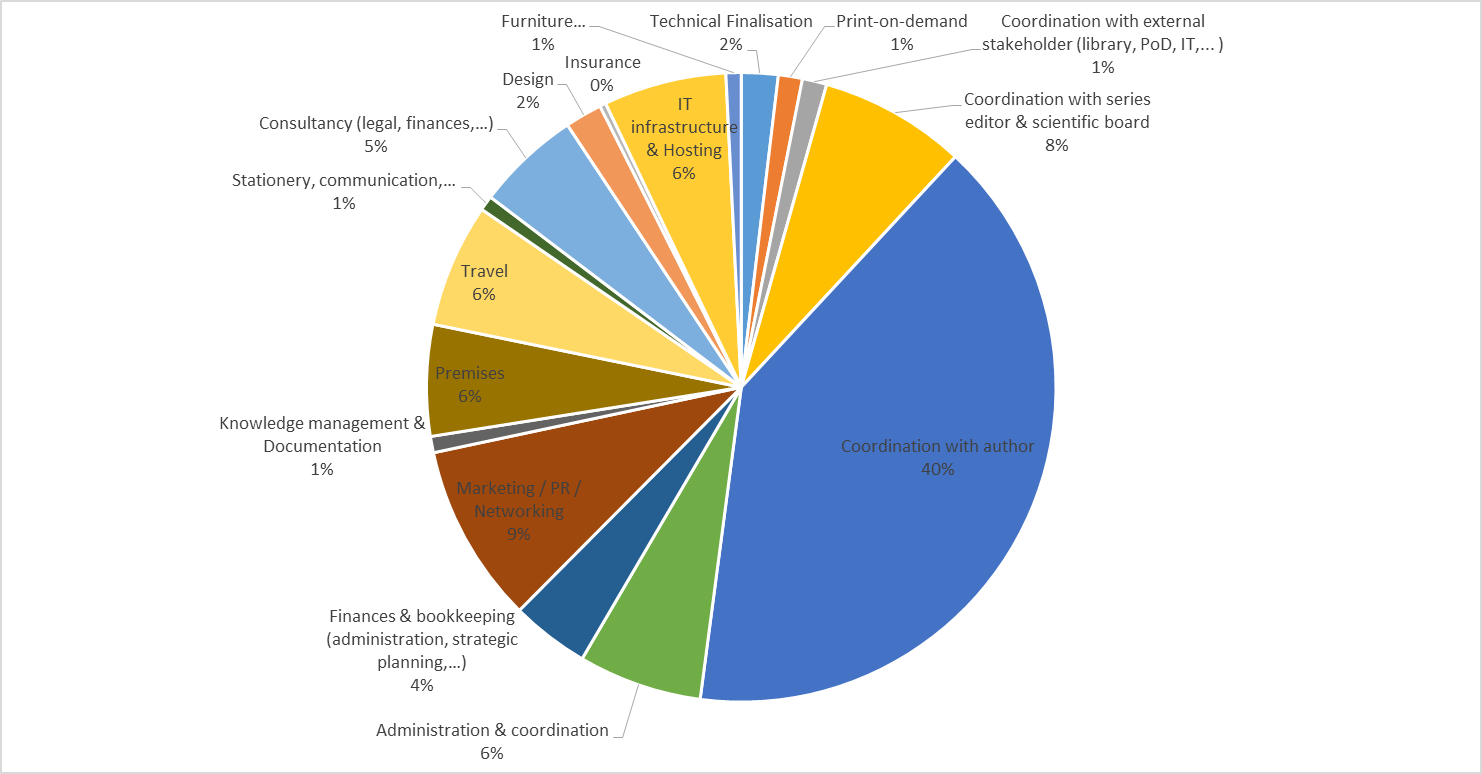
\includegraphics[width=\textwidth]{img/Kuchen.png}
\caption{Aufteilung der Kosten zwischen Koordination (rechts) und allem
anderen (links)}
\end{figure}

\hypertarget{inventarisierung-der-einnahmequellen}{%
\subsection{Inventarisierung der
Einnahmequellen}\label{inventarisierung-der-einnahmequellen}}

Analog zu den Ausgaben kann man auch bei den Einnahmemöglichkeiten
verfahren. Auch hier ist als erstes eine Inventarisierung der möglichen
Einnahmearten angebracht. Wer soll wie an den Kosten beteiligt werden?
Leser über Freemium, Autoren über Gebühren, Bibliotheken über
Mitgliedschaften, Forschungsförderer über Projektmittel?

\hypertarget{bezifferung-der-projizierten-einnahmen}{%
\subsection{Bezifferung der projizierten
Einnahmen}\label{bezifferung-der-projizierten-einnahmen}}

In gleicher Weise können nun den einzelnen Einnahmequellen Größen
zugeordnet werden. Hierbei handelt es sich zuerst um Schätzungen, die
dann später mit den tatsächlich erzielten Einnahmen abgeglichen werden
können.

\hypertarget{veruxf6ffentlichung-der-einnahmen}{%
\subsection{Veröffentlichung der
Einnahmen}\label{veruxf6ffentlichung-der-einnahmen}}

In dem Blogpost von OBP finden wir folgende Einnahmen:

\begin{itemize}
%\tightlist
\item
  \emph{Sales} (82.873 USD),
\item
  \emph{Title grants} (68.396 USD),
\item
  \emph{Library membership} (30.986 USD) und
\item
  \emph{OBP grants} (15.708 USD).
\end{itemize}

Ungefähr 40\,\% entfallen also auf den Verkauf, während fast der gleiche
Wert auf Grants entfällt.

\hypertarget{zusammenfassung-offene-buchhaltung}{%
\subsection{Zusammenfassung offene
Buchhaltung}\label{zusammenfassung-offene-buchhaltung}}

Um für die allgemeine Öffentlichkeit Transparenz hinsichtlich der Kosten
der Monographieproduktion herzustellen, müssen also Kosten sowie
Einnahmen erstmal gelistet werden, dann beziffert, und schließlich zur
Nachnutzung veröffentlicht werden (idealerweise als CC0-lizenzierter
Datensatz). Die Auflistung der verschiedenen Kosten/Einkommensarten
läuft im allgemeinen gut, bei der Bezifferung und Aufschlüsselung sieht
es schon anders aus. Verschiedene Universitätsverlage weisen diese zum
Beispiel noch nicht einmal intern aus. Die Veröffentlichung derartiger
Zahlen schlussendlich ist eindeutig noch ein Desideratum, und nur
vereinzelt finden sich etwas genauere Aufschlüsselungen, wie zum
Beispiel von OBP.

(Offensichtliche Analogien ergeben sich hier zu dem OpenAPC-Projekt im
Zeitschriftenbereich: \url{https://treemaps.intact-project.org/})

\hypertarget{das-projekt-full-disclosure}{%
\section{\texorpdfstring{Das Projekt \emph{Full
Disclosure}}{Das Projekt Full Disclosure}}\label{das-projekt-full-disclosure}}

Das OpenAire-Programm der EU hat im letzten Jahr einen Call zu
\emph{Alternative Funding Mechanism for non-author fee based Open Access
Publishing} veröffentlicht. In dessen Rahmen wurde das Projekt
\enquote{Full disclosure: replicable strategies for book publications
supplemented with empirical data} von Language Science Press mit 18.500
EUR gefördert. Ziel ist hier, das Geschäft von Language Science Press
genau zu beschreiben, um so eine Nachnutzung/Replizierung zu
ermöglichen. Dies umfasst sowohl die qualitative Perspektive, wie zum
Beispiel Arbeitsabläufe, wie auch die quantitative Perspektive:
Geschäftszahlen.

Folgende Dokumente liegen nun vor:

\begin{enumerate}
\def\labelenumi{\arabic{enumi}.}
%\tightlist
\item
  Das Geschäftsmodell von 2015 mit einer Evaluation aus dem Jahr 2018
\item
  Die Geschäftszahlen aus dem Jahr 2017
\item
  Eine granulare Tabellenkalkulation über fünf Jahre mit insgesamt 100
  Variablen für Kosten und Einnahmen
\item
  Ein \enquote{Kochbuch} für die qualitativen Aspekte, von der
  Rechtsform bis zum Community Building.
\end{enumerate}

\hypertarget{geschuxe4ftsmodell}{%
\subsection{Geschäftsmodell}\label{geschuxe4ftsmodell}}

Im Jahr 2015 entwickelte eine Betriebswirtschaftlerin ein
Geschäftsmodell für die Verstetigung von Language Science Press über
fünf Jahre, das zur Vorlage an die Leitung der Freien Universität Berlin
bestimmt war. Dieses Geschäftsmodell folgt einer üblichen Blaupause mit
Analyse des Produkts, der Kunden, des Wertversprechens, der
Einnahmearten. Weiterhin werden Aufwände in Zeit und Geld,
Personalbedarf und Kostendeckungsbeiträge verschiedener Einnahmearten
projiziert.

Das Modell hat den Vorteil, dass es auf einer qualitativen Grundlagen
die erwarteten Werte in Bezug auf Kosten und Einnahmen quantifiziert.
Rückblickend kann man sagen, dass die Erwartungen weit von der Realität
entfernt waren. Beispielsweise stehen im Geschäftsmodell
Spendeneinnahmen von 9.600 EUR, realisiert wurden jedoch nur 2.500 EUR.
Aber gerade durch die quantifizierten Vorhersagen ergeben sich hier
interessante Erkenntnisse. Die einzelnen Abschnitte des Geschäftsmodells
werden mit den tatsächlich realisierten Kosten/Einnahmen verglichen und
mögliche Alternativen werden aufgezeigt.

\hypertarget{geschuxe4ftszahlen-aus-dem-jahr-2017}{%
\subsection{Geschäftszahlen aus dem Jahr
2017}\label{geschuxe4ftszahlen-aus-dem-jahr-2017}}

Die folgenden Zahlen stehen als csv-Dateien zum Download zur Verfügung:

\begin{itemize}
%\tightlist
\item
  Zugriffszahlen auf der eigenen Webseite, GoogleBooks, DOAB
\item
  Printverkäufe
\item
  Spendeneinnahmen
\item
  Mitgliedschaftseinnahmen
\item
  Ausgaben (Personal, Reisen, Rechtsbeistand, ...)
\end{itemize}

Die Personalausgaben sind allerdings nicht den einzelnen
Tätigkeitsfeldern zugeordnet, da eine entsprechende granulare
Zeiterfassung nicht vorgenommen wurde.

\hypertarget{tabellenkalkulation}{%
\subsection{Tabellenkalkulation}\label{tabellenkalkulation}}

Um die Personalausgaben besser Tätigkeiten zuordnen zu können, wird die
interne Tabellenkalkulation mit 100 Variablen veröffentlicht. Die
Variablen beginnen mit der projizierten Anzahl Veröffentlichungen pro
Jahr und gehen dann über die erwarteten Printverkäufe, die Anzahl
Spender und den durchschnittlichen Spendenbetrag zu dem zeitlichen
Aufwand, der verschiedenen Aufgaben zugemessen wird: Autorenbetreuung,
Korrektorat, Textsatz, Koordination mit Dienstleistern, Dokumentation,
Lobbying et cetera. Die einzelnen Aufgaben sind jeweils einer
Beschäftigtengruppe zugeordnet (Professur, Postdoc, Sekretariat,
Hilfskraft). Aus dem tariflichen Gehalt können so die Personalkosten
ermittelt werden, die dann auf die veröffentlichten Bücher umgelegt
werden. So ergibt sich ein kalkulatorischer Preis pro Buch. Ebenfalls
können Korrektorat und Satz outgesourct werden. Dadurch verringert sich
der interne Personaleinsatz, aber die externen Kosten pro Buch erhöhen
sich. Die Tabellenkalkulation läuft über fünf Jahre. Die Annahme ist,
dass kein Projekt länger als fünf Jahre defizitär betrieben werden wird.

\hypertarget{kochbuch}{%
\subsection{Kochbuch}\label{kochbuch}}

Das Kochbuch beinhaltet Grundlagen der Community-basierten
Buchproduktion, Tipps und Tricks, Fallstricke sowie Lessons Learned und
ist als qualitative Ergänzung der Kalkulationen gedacht.

\hypertarget{einsichten}{%
\section{Einsichten}\label{einsichten}}

Der Vorteil eines quantifizierten Modells ist, dass man es mit der
Realität abgleichen kann. Hier der Abgleich für das Jahr 2017:

\pagebreak

\begin{longtable}[]{@{}lll@{}}
\toprule
Quelle & Soll & Ist\tabularnewline
\midrule
\endfirsthead
\toprule
Quelle & Soll & Ist\tabularnewline
\midrule
\endhead
Printmarge & 24.000\,€ & 5.977\,€\tabularnewline
BPCs & 48.000\,€ & 2.500\,€\tabularnewline
Institutionelle Mitgliedschaften & 56.000\,€ & 0\,€
(85.000\,€²⁰¹⁸)\tabularnewline
Spenden & 9.600\,€ & 2.500\,€\tabularnewline
Mitgliedsbeiträge & 13.200\,€ & 120\,€\tabularnewline
Kontext: veröffentlichte Titel & 48 & 26\tabularnewline
\bottomrule
\caption{Erwartete Einnahmen und De-facto-Einnahmen Language Science
Press in 2017}
\end{longtable}

Man erkennt mühelos, dass das ursprüngliche Modell überhaupt in 4/5 der
Fälle überhaupt nicht tragfähig war. Die 85.000 EUR durch
Institutionelle Mitgliedschaften fallen ebenfalls erst im Jahr 2018 an,
übertreffen aber die kalkulierten Einnahmen und stellen für sich allein
mehr als siebenmal soviel wie alle anderen Einnahmearten zusammen.

Verglichen mit den Zahlen von OBP aus 2015, die 40\,\%
Kostendeckungsbeitrag durch Printverkäufe zeigten, ergibt sich hier also
ein vollkommen anderes Bild: Die Printmarge kann keinen wesentlichen
Beitrag leisten. Die eindeutige Schlussfolgerung aus diesen Zahlen ist,
dass eine Finanzierung über Institutionelle
Mitgliedschaften/Konsortialmodelle am vielversprechendsten ist. Man kann
darüber hinaus durchaus die Frage stellen, ob man auf die anderen
Einkommensarten nicht komplett verzichten kann, um das Modell noch
weiter zu vereinfachen. Diese Erkenntnis ist intern bei Language Science
Press schon länger verbreitet, durch die Veröffentlichung der Zahlen
können jetzt aber auch andere Projekte davon profitieren. Die
Soll-Ist-Analyse ist allerdings nur möglich, weil das Soll vorher
bereits beziffert wurde.

Auf der Ausgabenseite finden sich 76.054 EUR an Personalkosten.
Verglichen damit sind alle anderen Ausgabenarten nebensächlich. Eine
Erhöhung/Senkung der Personalkosten hat also einen wesentlichen Einfluss
auf die Kosten pro Titel. Eine minutengenaue Aufschlüsselung der
Tätigkeiten der Angestellten liegt nicht vor, wie schon oben erwähnt
entfällt aber der Löwenanteil auf die Autorenbetreuung. Jede
Vereinfachung in diesem Bereich schlägt sich also signifikant nieder.
Dazu gehören deutlichere Dokumentation (Handreichungen, Screencasts),
bessere Templates, Tools zur Unterstützung der Autoren bei der
richtliniengetreuen Erstellung von Manuskripten. Ein nicht zu
unterschlagender Aspekt ist, dass der Koordinator von Language Science
Press die wesentlichen Bereiche Autorenbetreuung, Textsatz und
Serveradministration aus einer Hand abdecken kann und daher keine
Koordinationskosten oder Reibungsverluste zwischen Teammitgliedern
anfallen.

Im Jahr 2017 veröffentlichte Language Science Press 26 Titel. Auf Basis
der vorliegenden Zahlen ergeben sich aufs Neue kalkulatorische Kosten
pro Titel zwischen 3000 und 4000 EUR. Ab 2018 wird Raummiete als
Kostenposten dazukommen, so dass die Zahl sich den 4000 nähern wird.

Als abschließende Erkenntnis sei noch angemerkt, dass fast alle
verlagsseitigen Kosten bei der Aufbereitung des Manuskripts für den
Druck anfallen:

\begin{itemize}
%\tightlist
\item
  Die Forschungsleistung kostet den Verlag nichts.
\item
  Die Erstellung der eingereichten Version kostet den Verlag nichts.
\item
  Die Begutachtung wird von den Reihen organisiert und kostet den Verlag
  nichts.
\item
  Die Überarbeitung des Manuskripts durch die Autorin kostet den Verlag
  nichts.
\item
  \textbf{Die Aufbereitung des Manuskripts in Zusammenarbeit mit der
  Autorin verursacht wesentliche Kosten.}
\item
  Die digitale Distribution kostet pro Buch minimal (Aufwand 1--2
  Stunden).
\item
  Druck und Vertrieb kosten den Verlag in Zeiten von print-on-demand
  quasi nichts (Aufwand \textless1 Stunde).
\item
  Lagerhaltung entfällt.
\item
  Archivierung bei Zenodo kostet den Verlag nichts.
\end{itemize}

\hypertarget{warum-kostet-ein-wissenschaftliches-buch-denn-nun-28.000-eur}{%
\section{Warum kostet ein wissenschaftliches Buch denn nun 28.000
EUR?}\label{warum-kostet-ein-wissenschaftliches-buch-denn-nun-28.000-eur}}

Die Eingangsfrage dieses Artikels war \enquote{Warum kostet ein
wissenschaftliches Buch 28.000 EUR?} Um diese Frage zu beantworten,
müssen wir wissen, was eigentlich genau produziert wird, welche
Tätigkeiten damit verbunden sind, und mit wieviel diese Tätigkeiten zu
Buche schlagen. Die Frage, warum ein Buch nun 28.000 EUR kostet, kann
vermutlich nur John Sherer beantworten, ich hoffe aber, dass ich in
diesem Artikel darlegen konnte, warum Language Science Press auf
kalkulatorische Kosten von 3.500 EUR pro Buch kommt.

Durch die Veröffentlichung des Geschäftsmodells, der Kalkulationsmethode
und der Zahlen können andere Projekte jetzt feststellen, was sie
gleich/anders machen, und wie sie daher auf höhere/niedrigere Kosten
kommen. Hierbei ist das Ziel allerdings nicht Pfennigfuchserei, sondern
ein realistischer Einblick in die Unterschiede zwischen Disziplinen.
Meine Vermutung wäre, dass zum Beispiel in der Philosophie die Texte im
Allgemeinen typographisch weniger anspruchsvoll sind als in der
Sprachwissenschaft und daher der Aufwand pro Buch auch geringer sein
sollte. Auf der anderen Seite würde ich bei der Kunstgeschichte von
höheren Kosten pro Band ausgehen. Um diese Vermutung zu belegen,
brauchen wir aber ebenfalls vergleichbare Zahlen aus diesen Disziplinen.

Mit TTOA gibt es diese Bestrebungen bereits für den Zeitschriftenbereich
auf Verlagsseite (interessanterweise bei Kosten von 1.400 EUR pro
Artikel), mit dem OpenAPC-Projekt als Widerpart bei den Bibliotheken.
Ziel ist, ähnliches auch für die Buchproduktion zu etablieren. Ubiquity
Press oder Open Book Publishers weisen bereits gewisse Zahlen aus. Für
einen Open-Access-Verlag sollte es selbstverständlich sein, neben den
Büchern und der verwendeten Software auch die Geschäftsprozesse und
Workflows zur Nachnutzung freizugeben, ergänzt um die tatsächlichen
Geschäftszahlen. Jean-Sébastien Caux hat hierfür in Abgrenzung zu
\enquote{Gold OA} und APC-freiem \enquote{Platinum OA} den Begriff
\enquote{Palladium OA} geprägt (Caux 2017). Ein Palladium-OA-Verlag wird
von ihm definiert als

\begin{quote}
\enquote{\textbf{Palladium {[}Pd{]}} publisher runs a purely
not-for-profit public enterprise: none of its activities generate any
profit, and all financial statements are publicly disclosed}
\end{quote}

Wie im vorigen Abschnitt dargelegt, entstehen eigentlich nur bei der
Aufbereitung des Manuskripts wesentliche Kosten im Verlag. Wenn Verlage
nun also auf kalkulatorische Kosten von bis zu 129.000 USD kommen, haben
sie also entweder eine sehr aufwendige Aufbereitung, oder aber sie geben
Geld in anderen Bereichen aus, wo das aus meiner Sicht nicht angezeigt
ist, beispielsweise Lagerhaltung oder Vertrieb über einen eigenen
Webshop. Auch hier kann Transparenz helfen. Die Entscheidung, dass die
Kostenstruktur veröffentlicht wird, sollte recht automatisch zu einem
Überdenken der einzelnen Posten führen.

Warum kostet ein wissenschaftliches Buch nun 28.000 EUR? Ich weiß es
nicht und es erschließt sich mir nicht. Ich weiß aber, dass alle
Open-Access-Verlage davon profitieren werden, wenn sie ihre
Kostenstrukturen im Rahmen von \emph{Offenen Büchern} teilten. Mit dem
Projekt \emph{Full Disclosure} ist hier ein Anfang gemacht. Es ist nicht
davon auszugehen, dass Language Science Press mit seinem Modell im
ersten Anlauf den Stein der Weisen gefunden hat, daher bitte ich um rege
Kritik des Ansatzes und um die Veröffentlichungen weiterer Zahlen, auf
dass sich ein empirischer Vergleich anstellen lasse.

\hypertarget{dokumente}{%
\section{Dokumente}\label{dokumente}}

Das Geschäftsmodell von Language Science Press steht auf PaperHive zum
\enquote{Collaborative Reading} bereit:
\url{https://paperhive.org/documents/items/fDiLi_1bkqDQ}.

Das Kochbuch findet sich auf
\url{https://paperhive.org/documents/items/RoiQzwhr4uRT}.

Die Geschäftszahlen finden sich auf
\url{https://github.com/langsci/opendata}.

\hypertarget{literatur}{%
\section{Literatur}\label{literatur}}

Adema, Janneke \& Stone Graham. 2017. Changing publishing ecologies: A
landscape study of new university presses and academic-led publishing.
\url{http://repository.jisc.ac.uk/6666/1/Changing-publishing-ecologies-report.pdf}

Anderson, Kent. 2018. Focusing on Value --- 102 Things Journal
Publishers Do (2018 Update). Scholarly Kitchen, 06.02.2018.
\url{https://scholarlykitchen.sspnet.org/2018/02/06/focusing-value-102-things-journal-publishers-2018-update/}.

Caux, Jean-Sébastien. 2017. Noble metals for a noble cause. 20.09.2017.
\url{https://jscaux.org/blog/post/2017/09/20/noble-metals-noble-cause/}.

Ferwerda, Eelco et al.~2017. A landscape study on open access and
monographs: policies, funding and publishing in eight European
countries. Knowledge Exchange.
\url{https://doi.org/10.5281/zenodo.815932}.

Gatti, Rupert. 2015. Introducing Data to the Open Access Debate: OBP's
Business Model (Part Three). Open Book Publishers Blog, 15.10.2015.
\url{https://doi.org/10.11647/OBP.0173.0016}.

Maron, Nancy L. et al.~2016. The costs of publishing monographs: Toward
a transparent methodology DOI: \url{https://doi.org/10.18665/sr.276785}
.

Nordhoff, Sebastian. 2015. What's the cost of an open access book?
Language Science Press Blog, 29.09.2015.
\url{https://userblogs.fu-berlin.de/langsci-press/2015/09/29/whats-the-cost-of-an-open-access-book/}.

Sherer, John. 2018. Open Access History Monograph Initiative. Longleaf
Services Blog, 13.06.2018.
\url{http://www.longleafservices.org/blog/oa-monographs/}.

%autor
\begin{center}\rule{0.5\linewidth}{\linethickness}\end{center}

\textbf{Sebastian Nordhoff} ist promovierter Linguist und
Geschäftsführer von Language Science Press. Vor dem Aufbau von Language
Science Press lag sein Schwerpunkt auf Sprachkontakt in Paraguay und Sri
Lanka. Im Rahmen von Open Access, Open Science, Open Data, Open
Everything hat er unter anderem zu Linguistic Linked Open Data
gearbeitet sowie die bibliographische Web-Plattform glottolog.org zu
sprachlicher Diversität mitentwickelt. Kontakt:
\url{mailto:sebastian.nordhoff@langsci-press.org}

\end{document}
